\section{Real Robot System Setup}
\label{sec:body}
Our real robot is built on the TIANJI M6 and WUJI Hand, as shown in Fig.~\ref{fig:body}.
The policy’s inference frequency is set at 50 Hz. The commands are sent with a delay kept between 18 and 30 milliseconds. The low-level interface operates at a frequency of 500 Hz, ensuring smooth real-time control. The communication between the control policy and the low-level interface is realized through LCM (Lightweight Communications and Marshalling).



\begin{figure}
  \centering
    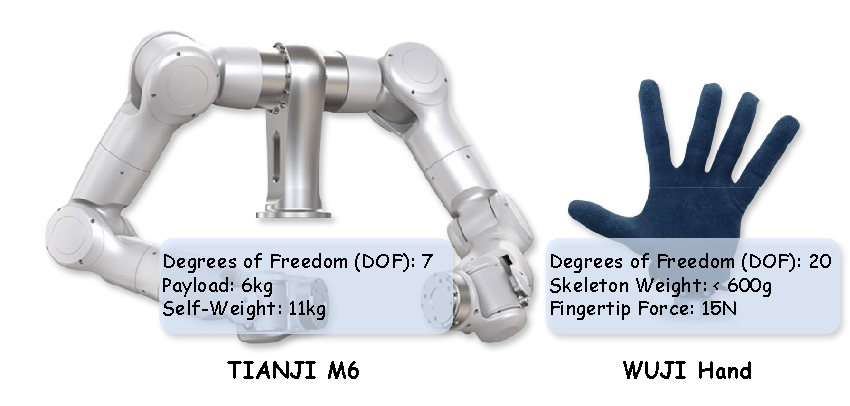
\includegraphics[width=\linewidth]{Fig/body.pdf}\\
  \caption{\textbf{Standardized Experimental Platform.} All real-world experiments are conducted on a unified hardware configuration consisting of the TIANJI M6 7-DOF robotic arm and the 20-DOF WUJI dexterous hand. This integrated system provides the high-precision control and high-dimensional actuation space required for complex manipulation tasks.}
  \label{fig:body}
\end{figure}



We collect real-world demonstration data through a teleoperation system, as shown in Fig.~\ref{fig:operator}. Our hardware setup consists of dual Tianji 7-DOF robotic arms and dual Wuji 20-DOF dexterous hands, yielding a total of 54 degrees of freedom.                            

For arm control, the human operator wears five HTC Vive trackers (mounted on the chest, both wrists, and both upper arms). The system computes wrist-to-chest relative transforms at 100-120 Hz and feeds them into a Pinocchio-based inverse kinematics solver running in a separate process. The resulting joint commands are further smoothed by a Ruckig trajectory generator with velocity, acceleration, and jerk constraints before being sent to the robot arms at 200 Hz.                  

For hand control, the operator wears Manus data gloves. The raw glove signals are converted to a 21-point MediaPipe hand skeleton format and retargeted to the 20-DOF Wuji hand joint space via a dedicated retargeting module, with an exponential moving average filter applied for motion smoothing.


\begin{figure}
  \centering
    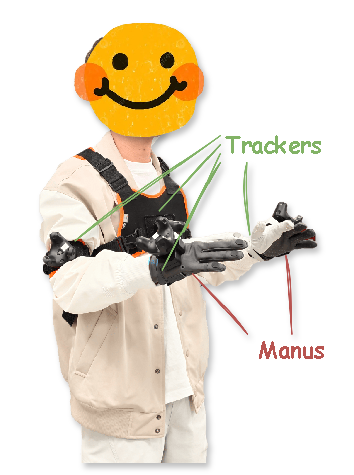
\includegraphics[width=0.45\linewidth]{Fig/operator.pdf}\\
  \caption{Operator to collect real world data.}
  \label{fig:operator}
\end{figure}






















\section{Additional Details on Evaluation Metrics}
\label{sec:metric}
This section provides technical definitions and implementation details for all evaluation metrics used in our experiments.      

\subsection{Generative Quality}
We adopt a subset of task-aligned metrics from PAI-Bench~\citep{zhou2025pai} to assess the visual and temporal quality of generated videos:
\begin{itemize}[labelsep=0.6em, leftmargin=1.2em,itemindent=0em]
\item \textbf{Imaging Quality (IQ):} Evaluates low-level visual fidelity including clarity, noise levels, and compression artifacts. We employ the MUSIQ~\citep{ke2021musiq} predictor trained on the SPAQ dataset to compute a frame-level perceptual quality score.
\item \textbf{Motion Smoothness (MS):} Quantifies temporal coherence and physical plausibility of motion dynamics. It is computed as the reconstruction error between generated frames and those synthesized via the AMT-S~\citep{li2023amt} frame interpolation model, where lower interpolation error indicates smoother motion.
\item \textbf{Subject Consistency (SC):} Measures the identity stability of the primary subject across the video sequence. We compute the mean pairwise cosine similarity of DINO~\citep{zhang2022dino} ViT-B/16 features between the first frame and all subsequent frames.
\item \textbf{I2V-Subject (Subj.):} For image-to-video generation, this metric evaluates how faithfully the model preserves the identity of the input reference image throughout the generated sequence. It is computed as the DINO feature similarity between the conditioning image and each generated frame.  
\item \textbf{PSNR (Peak Signal-to-Noise Ratio):} Measures pixel-wise reconstruction accuracy between generated and GT frames. Higher values indicate lower distortion. We report the mean PSNR across all frames (excluding the shared first frame) and all video samples. 
\item \textbf{SSIM (Structural Similarity Index):} Evaluates the preservation of structural information by jointly considering luminance, contrast, and structural components between generated and GT frame pairs. 
\item \textbf{LPIPS (Learned Perceptual Image Patch Similarity):} Measures perceptual distance between generated and GT frames using deep features from a pre-trained AlexNet. Lower values indicate higher perceptual similarity, and LPIPS is generally better aligned with human visual judgments than pixel-level metrics. 
\end{itemize}                                                                                                  


\subsection{Geometric Accuracy}
For methods that jointly predict depth maps, we evaluate structural fidelity of the estimated geometry using scale-invariant depth metrics:
\begin{itemize}[labelsep=0.6em, leftmargin=1.2em,itemindent=0em]
\item \textbf{Absolute Relative Error (AbsRel $\downarrow$):} Measures the mean relative deviation between the predicted depth $\hat{d}$ and ground-truth depth $d^*$. Since different methods may produce depth in arbitrary scales, we first perform scale-invariant alignment via median scaling: $s = \text{median}(d^*) / \text{median}(\hat{d})$, then compute:
\begin{equation}
\text{AbsRel} = \frac{1}{|\mathcal{V}|} \sum_{p \in \mathcal{V}} \frac{|s \cdot \hat{d}_p - d^*_p|}{d^*_p},
\end{equation}
where $\mathcal{V}$ denotes the set of valid pixels ($d^* > 0$).
\item \textbf{Threshold Accuracy ($\boldsymbol{\delta_1 < 1.25}$ $\uparrow$):} Reports the percentage of pixels whose depth ratio falls within a tolerance threshold:
\begin{equation}
\delta_1 = \frac{1}{|\mathcal{V}|} \sum_{p \in \mathcal{V}} \mathbb{1}\left[\max\left(\frac{s \cdot \hat{d}_p}{d^*_p},\; \frac{d^*_p}{s \cdot \hat{d}_p}\right) < 1.25\right].
\end{equation}
Higher values indicate better geometric alignment with the ground truth.
\end{itemize}


\subsection{Motion Consistency}
For methods that predict optical flow, we evaluate the temporal dynamics accuracy:
\begin{itemize}[labelsep=0.6em, leftmargin=1.2em,itemindent=0em]
\item \textbf{Average End-Point Error (AEPE $\downarrow$):} Measures the accuracy of predicted optical flow fields against ground-truth flow. For each pixel $p$ with predicted flow $\hat{\mathbf{f}}_p = (\hat{u}_p, \hat{v}_p)$ and ground-truth flow $\mathbf{f}^*_p = (u^*_p, v^*_p)$, the end-point error is defined as:
\begin{equation}
\text{AEPE} = \frac{1}{|\mathcal{V}|} \sum_{p \in \mathcal{V}} \left\| \hat{\mathbf{f}}_p - \mathbf{f}^*_p \right\|_2 = \frac{1}{|\mathcal{V}|} \sum_{p \in \mathcal{V}} \sqrt{(\hat{u}_p - u^*_p)^2 + (\hat{v}_p - v^*_p)^2}.
\end{equation}
Since both predicted and ground-truth optical flow are stored as color-coded visualizations using the Middlebury color wheel encoding, we compute the AEPE as the per-pixel $\ell_2$ distance in the normalized RGB color space between the predicted and ground-truth flow maps. The metric is averaged over all valid frames (excluding the first frame, which has no temporal reference) and all video samples. Lower AEPE indicates more accurate motion prediction.
\end{itemize}  







\section{Preliminaries}
\label{sec:method:preliminaries}
Our study builds upon the Wan family of video generation models~\citep{wang2025wan}, a latent video diffusion transformer capable of generating temporally coherent video from a single input image or text prompt. The model consists of a 3D variational autoencoder $(\mathcal{E}, \mathcal{D})$ and a transformer-based diffusion model parameterized by $\Theta$. Given an input latent $z_0 = \mathcal{E}(V_0)$, the forward process follows the rectified flow formulation~\citep{esser2024scaling}, where the noised latent is generated by linear interpolation:
\begin{equation}
z_t = (1 - t)\, z_0 + t\,\epsilon, \quad \epsilon \sim \mathcal{N}(0, I)
\label{eq:zt_interp}
\end{equation}
with timestep $t \in [0, 1]$. The denoising process learns a velocity field $v_\Theta(z_t, t)$ that guides the transformation of noise back to data. The model is trained using a conditional flow matching~\citep{lipman2022flow}, with objective:
\begin{equation}
\mathcal{L}_{\text{CFM}} =
\mathbb{E}_{t, z_0, \epsilon}\!\left[\left\lVert
v_\Theta(z_t, t) - u_t(z_0 \mid \epsilon)
\right\rVert_2^2\right]
\label{eq:l_cfm}
\end{equation}
where $u_t$ is the target velocity derived analytically from the forward process. At inference, a sequence of latent frames is recovered by integrating $v_\Theta$ over time.

In the image-to-video (I2V) setting, the model is conditioned on an initial image $I_0$ encoded as $z_{\text{img}} = \mathcal{E}(I_0)$. The transformer-based denoiser $\mathcal{F}_\Theta$ autoregressively predicts video latents $\{z^{(f)}\}_{f=1}^F$, starting from $z_{\text{img}}$ and producing temporally consistent sequences. In the text-to-video (T2V) setting, the model is instead conditioned on a text prompt $p$ encoded as $z_{\text{text}}=\mathcal{T}(p)$ and starts the autoregressive generation from noise. The final video is reconstructed as $\hat{V} = \mathcal{D}(z^{(1)}, \dots, z^{(F)})$.




\section{Baseline Implementation Details} 

\noindent 
\textbf{Free4D.}
Free4D~\citep{liu2025free4d} lifts a single image into a dynamic 4D Gaussian Splatting (4DGS) representation. Given the first frame of each ground-truth video as input, we run the full Free4D pipeline: (1) the built-in ViewCrafter module with DUSt3R-based monocular depth estimation synthesizes 25 novel views from the input image via a video diffusion model at $576 \times 1024$ resolution; (2) COLMAP sparse reconstruction estimates camera poses and produces a sparse point cloud for Gaussian initialization; (3) the 4DGS model with HexPlane-based deformation fields is optimized for 10{,}000 iterations (3{,}000 static initialization + 7{,}000 joint optimization), with temporal resolution $[64, 64, 64, 150]$; (4) RGB and depth videos are rendered from the original camera viewpoint across all timesteps. Since the rendered depth is in arbitrary scale, we apply per-frame median scaling alignment before computing depth metrics.                                            

\noindent 
\textbf{4DNeX.}
4DNeX~\citep{chen20254dnex} is a feed-forward 4D scene generation framework that repurposes the Wan2.1-I2V-14B~\citep{wang2025wan}, fine-tuned with learnable domain embeddings and LoRA adapters, to jointly produce RGB appearance and per-pixel XYZ point-cloud geometry from a single image and a text prompt. We adopt the official variant, using the provided 4dnex-lora weights (rank $64$, fused at scale $0.5$).   
For each sequence we extract the first frame of the ground-truth video as the conditioning image and use the corresponding caption, appending the official \texttt{POINTMAP\_STYLE.} suffix as required by the released model. For each sample we run $50$ denoising steps with classifier-free guidance scale $5.0$ and seed $42$, generating $49$ frames at $24$~fps. We obtain the depth video by taking the $z$-channel of the predicted pointmap, min--max normalized per sequence to $[0, 255]$. 

\noindent 
\textbf{TesserAct.}
TesserAct~\citep{zhen2025learning} is built upon CogVideoX-5b-I2V~\citep{yang2024cogvideox} and fine-tuned to jointly generate RGB, depth, and surface normal videos from a single initial frame and a language instruction. We adopt the official  checkpoint. Since TesserAct requires depth and normal maps as additional conditioning inputs, we first extract the initial RGB frame from each ground-truth video, then apply network to estimate monocular depth and surface normals. The three modalities are concatenated along the channel dimension to form a 9-channel input. We generate 49 frames at $640\times480$ resolution using 50 DDPM denoising steps with guidance scale 7.5, image guidance scale 1.5. The model outputs RGB, depth, and normal videos concatenated along the width axis; we split along width to obtain separate RGB and depth predictions for evaluation. 


\section{Additional Qualitative Visualizations via RynnWorld-4D}
\label{appendix:rynnworld_4d}
To further showcase the generation quality of \our, we provide extended paired visualizations of \textbf{RGB}, \textbf{Depth}, and \textbf{Optical Flow} generated via RynnWorld-4D (Fig.~\ref{fig:rynnworld_4d_vis}). \our synchronously predicts future RGB, depth maps, and optical flow from a single RGB-D observation. These results demonstrate: 

(i) \textbf{Cross-modal Consistency:} The geometric structures in depth maps and motion boundaries in optical flow are precisely aligned with the RGB textures. 

(ii) \textbf{Physical Fidelity:} The model accurately captures complex 4D dynamics, such as object displacements and multi-contact interactions, in both human-centric and robot-specific environments.

(iii) \textbf{Temporal Coherence:} The generated sequences maintain stability over time without significant flickering or structural morphing.



\begin{figure}
    \centering
    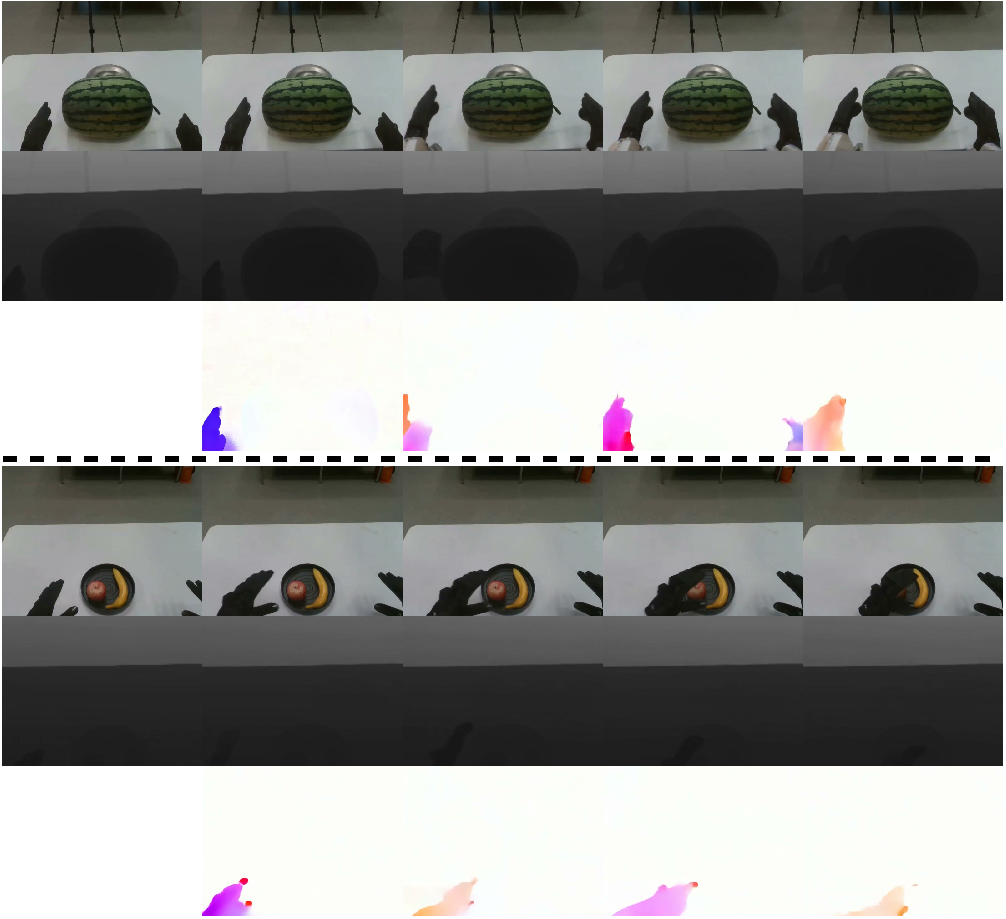
\includegraphics[width=1.0\textwidth]{Fig/appendix-vis.pdf}
    \caption{Extended qualitative results. Each row displays the generated RGB, depth, and optical flow sequences. The results highlight \our's ability to produce spatially and temporally coherent 4D predictions across various manipulation scenarios.}
    \label{fig:rynnworld_4d_vis}
\end{figure}
